\chapter{Разработка модели для нейро-нечеткого моделирования социально-экономических систем}

В данной главе описывается модифицированная модель
когнитивных карт с использованием рекуррентных нейросетей.
Производится выбор метрик оценки качества работы системы.

\section{Разработка нейро-нечеткой модели с использованием рекуррентный нейросетей}

Можно усовершенствовать модель TTR LSTM, рассмотренную в первой главе,
если вместо сетей прямого распространения использовать рекуррентные сети,
например, LSTM \cite{LSTM_paper}. Такую модель будем называть FCM-LSTM \ref{img:nfcm_compare_with_classif_fcm}.
Выбор рекуррентных сетей обусловлен тем, что такие сети позволят естественно сохранять информацию об
истории концептов в своем скрытом состоянии. В то время как для
того, чтобы учитывать значения концептов на предыдущих итерациях
в сетях прямого распространения, каждый предыдущий шаг должен быть
описан как отдельный параметр. Это сильно увеличивает количество параметров
модели и усложняет ее обучение.

\def\figurename{Рис}
\begin{figure}[t]
	\centering
	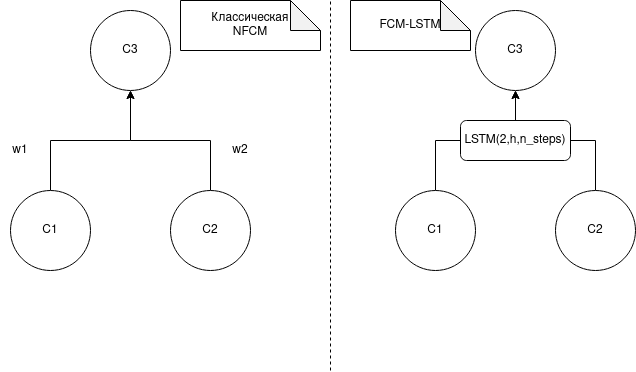
\includegraphics[height=7cm]{./img/fcm_lstm_scheme.png}
	\caption{Сравнение архитектуры классической когнитивной карты и FCM-LSTM. }
	\label{img:nfcm_compare_with_classif_fcm}
\end{figure}

\textbf{Сравнение FCM-LSTM с полносвязными сетями}:
У FCM-LSTM меньше параметров по сравнению с сетью прямого распространения,
которая бы учитывала больше количество предыдущих значений во временном ряде.
FCM-LSTM дольше обучается, но имеет значительно лучшую способность к предсказанию
на длинных временных рядах.
Модель будет дольше обучаться, потому что нельзя распараллелить
процесс обучения LSTM сетей, так как в сети учитывается, что внутреннее состояние меняется последовательно.
FCM-LSTM имеет лучшую интерпретируемость, так как содержит
экспертную информацию о взаимосвязи концептов.
Но для построения FCM-LSTM требуется эксперт, а как следствие,
ручная работа.

\textbf{Сравнение FCM-LSTM с TTR NFCM}:
FCM-LSTM дольше обучается, но на сложных наборах данных
может иметь более точные прогнозы.

\textbf{Сравнение FCM-LSTM с LSTM}:
LSTM сеть, которая бы соответствовала FCM-LSTM, будет иметь
больше параметров в случае, если граф FCM-LSTM не слишком
много связей. FCM-LSTM лучше интерпретируема.
Скорость обучения, при условии оптимизаций в FCM-LSTM, с
помощью которых обучение LSTM моделей в каждой вершине бы проходило
параллельно, будет примерно одинаковой.
Предсказательная способность должна быть лучше у FCM-LSTM.
Потому что такая модель более проста и структурирована.
LSTM модель может оказаться излишне усложненной, так как в ней будет
большое количество параметров.
Но для построения FCM-LSTM требуется эксперт, а как следствие,
ручная работа.
Для построения FCM-LSTM требуется эксперт.

Кроме того, так как карта представляет из себя ансамбль
более маленьких моделей, в случае ошибки в исходных данных
в одной части модели, можно переобучать не всю карту целиком,
а только ту часть в которой была ошибка. Так как процесс обучения
может занимать долгое время, эта оптимизация может существенно ускорить процесс.
Такой же прием можно применить и для случая, когда нужно дообучить карту на
новом наборе данных: можно дообучать карту частями.

\section{Построение FCM-LSTM}

Для того, чтобы создать модель, нужно определить параметры системы, концепты.
Каждый концепт будет соответствовать вершине графа карты.
После того, как концепты определены, нужно описать взаимодействие между концептами.
Одним из вариантов может быть полносвязный граф, когда каждый концепт имеет
влияние на каждый другой концепт. Теоретически, при увеличении количества
связей в модели, количество возможных зависимостей, которые она может описать
увеличивается. Однако, усложняется и сама модель так, что ее становится сложно обучить.
Слишком сложные модели легко переобучаются на тестовых данных.
Задача эксперта как раз заключается в том, что он должен
описать только необходимые и достаточные взаимосвязи.

Так же, как и большое количество взаимосвязей,
недостаточное количество связей или неверные связи, могут ухудшить
качество модели. Модель может оказаться недостаточно мощной, чтобы описать
исследуемый процесс. Поэтому важно найти именно существенные связи.

После того, как карта построена, необходимо "заморозить карту".
Это означает, что новые связи в карте больше появляться не будут.
Это необходимо для того, чтобы рассчитать параметры моделей, которые
лежат в каждой вершине графа карты: размерность данных на входе,
размерность внутреннего состояния, размерность данных на выходе модели.
Перед заморозкой для каждого концепта должна быть определена модель,
которая будет использована при моделировании данного концепта.

Для того, чтобы добавить новый концепт после заморозки карты,
потребуется переобучить карту. Как описано в предыдущем абзаце,
нет необходимости переобучать всю карту целиком. Нужно переобучить только
концепт, к которому добавилась новая связь.

После "заморозки", должны быть инициализированы модели в каждой вершине
карты. Эксперт имеет возможность задать создать любую модель заданной размерности
для каждого концепта отдельно. Выбор модели должен быть основан
на характере данных. Можно использовать как авторегрессионные модели,
так и нелинейные, в том числе и нейросетевые. Также можно использовать различные комбинации
этих подходов. В данной работе будет использоваться LSTM.

\section{Алгоритм обучения FCM-LSTM}

Каждый концепт имеет исторические данные, которые используются
для обучения модели концепта.

Процесс обучения можно разбить на несколько шагов:

\begin{itemize}
	\item Подготовка данных.
	\item Тренировка сети.
	\item Валидация обученной сети.
\end{itemize}

Подготовка данных. На этом этапе происходит разбиение
исторических данных на части для обучения и для валидации.
Это необходимо, чтобы не допустить переобучения сети:
когда на выборке для обучения показатели качества сети
отличные, но на валидационной выборке плохие.
В подготовку данных также нужно включить преобразование данных
в последовательности необходимой размерности. На вход
LSTM сеть принимает матрицу размерности $ seq\_len \times batch \times input\_size $.
$ seq\_len $ -~ длинна последовательности, непрерывный кусок данных.
$ batch $ -~ размер пакета на каждой итерации, для которого будет вычисляться градиент.
$ input\_size $ -~ количество связей, которые входят в обучаемый концепт.

Тренировка сети. На данном шаге происходит оптимизиция весов.
Для модель LSTM, соответствующая каждому концепту будет обучена
на данных, которые для данного концепта определил эксперт.
сети каждого концепта. В качестве функции потерь будет использоваться $ MSE $.
В качестве оптимизатора будет использован ADAM \cite{adam2014}.

Валидация сети подразумевает
проверку качества работы обученной сеты на данных,
которых не было в выборке для обучения.

\section{Алгоритм вычисления FCM-LSTM}

Алгоритм вычисления LSTM-NFCM не сильно отличается от
алгоритма вычисления классической нечеткой когнитивной карты.

Предсказание одной итерации в LSTM-NFCM ничем не будет отличаться
от предсказаний тех моделей, которые заложены в вершины графа.
Можно провести несколько итераций вычисления карты, с учетом вычисленных
данных. На следующем шаге модель будет обрабатывать данные,
которые сгенерировала на предыдущем шаге. Таким образом можно получить
более долгосрочное предсказание. Такой метод называется динамическое предсказание.

Кроме того, в такой модели должны проявиться влияния обратных связей, которые могут
быть заложены в архитектуре карты, если карта содержит циклы.
Таким образом, в LSTM-NFCM есть 2 уровня обратных связей:
на уровне модели концепта (LSTM) и на уровне структуры карты,
если карта содержит обратные связи.
Обратные связи на уровне структуры карты интересны тем, что
через них можно было бы выразить циклически меняющееся состояние системы.

Другой способ получить более долгосрочные предсказания -~ обучить LSTM
предсказывать на большее количество итераций вперед. Такой подход
требует больше памяти.

\section{Возможные проблемы алгоритма FCM-LSTM}

Так как в предложенной нейро-нечеткой модели
значительно усложнилась структура весов, то
анализ весов такой карты тоже заметно усложнился.
Вес влияния концептов в такой системе не статичен,
а зависит от истории изменения концептов, то есть
в разные моменты времени степень влияния одного концепта
на другой может быть разной.

Для обучения  нейросети требуется, чтобы
данные для обучения были репрезентативными. То есть
описывали все возможные значения, которые может принимать система.
Если в предсказании появляются данные, которых не было в обучающей выборке,
модель нужно переобучать. Можно предположить, что эту проблему можно решить,
если использовать версию LSTM без функции активации или, возможно, с другой
функцией активации, например, ReLU. ReLU просто вычислять. И в отличие от
сигмоиды, она не ограничена сверху. Также можно использовать другую модель.
При краткосрочном прогнозировании данный недостаток на является существенным.
Кроме того, такой проблемы можно избежать, если избавиться от тренда с
помощью интегрированной регрессионной модели так, чтобы на вход нейросети
поступал стационарный ряд.

Если внутреннее состояние будет иметь большую размерность,
модель будет потреблять много памяти. Возможно, модель можно
декомпозировать на меньшие задачи и обойтись несколькими концептами
с меньшей размерностью внутреннего состояния.
Но данный метод не относится к методам, в которых нужно бездумно
пользоваться готовой моделью, а нацелен на то, чтобы наоборот
получить больше понимания об изучаемом процессе.

При достаточно большом количестве временных рядов,
становится сложно экспертно определить взаимодействие между концептами.
Для задач с большим количеством рядов для исследования, без
модификаций, данный метод не будет эффективен. Так как потребует
большое количество вычислительных ресурсов.
Для таких задач можно использовать, например, градиентный бустинг \cite{friedman2002stochastic}.

\section{Выбор метрик для оценки качества работы моделей}

Кросс-валидация -~ это метод оценки модели на данных, не участвовавших
в обучении модели. Особенностью кросс-валидации для задачи прогнозирования
временных рядов заключается в том, перемешивать данные нельзя,
так как порядок данных во временном ряде -~ это его неотъемлемая составляющая.

В качестве критерия качества результата работы системы для предсказаний
для одного временного ряда, можно взять среднеквадратическую
масштабированную ошибку (RMSSE --- Root Mean Squared Scaled Error) \cite{hyndman2006another, shcherbakov2013survey}:

\begin{equation}\label{eq:rmsse}
	RMSSE = \sqrt{ \frac{ \frac{1}{h} \sum_{t=n+1}^{n+h}(Y_t - \hat{Y_t})^2  }{ \frac{1}{n-1} \sum_{t=2}^{n} (Y_t - Y_{t-1})^2 } }
\end{equation}

Данная метрика обладает рядом преимуществ:

\begin{itemize}
	\item Ошибка не зависит от масштаба и может быть эффективно использована для предсказаний временных рядов разных масштабов.
	\item Функция может быть вычислена безопасно. Деление на ноль может произойти только если временной ряд состоял из одного повторяющегося числа.
	\item Одинаково штрафуются и положительные, и отрицательные отклонения, метрика симметрична.
\end{itemize}

Для того, чтобы оценить получить ошибку по предсказанию для всех временных рядов,
можно использовать взвешенную среднеквадратическую масштабированную ошибку.
Она вычисляется по формуле:

\begin{equation}\label{eq:wrmsse}
	WRMSSE = \sum_{i=1}^{k} w_i * RMSSE_i
\end{equation}

Так как для некоторых значение $ RMSSE $ зависит от длины ряда, на котором обучается
модель, то для сравнения между собой моделей, обученных на выборках разной длины,
будет использоваться сумма квадратов ошибок:

\begin{equation}\label{eq:mse}
	MSE = \frac{1}{n} \sum_{i=1}^{n} (Y_i  - \hat{Y_i})^2
\end{equation}

\noindent Кроме того, в некоторых методах обучения
в процессе оптимизации весов будет использоваться именно эта метрика.


Для определения оптимальных гиперпараметров ARIMAX модели будет использоваться критерий Акаике \cite{sakamoto1986akaike, akaike, wagenmakers2004aic}.

Это критерий используется для сравнения одинаковых моделей с разными гиперпараметрами.
Чем меньше значение этого критерия, тем оптимальнее набор гиперпараметров.
Для случая, когда модели обучены на выборках одинаковой длины, этот критерий можно вычислить по формуле:

\begin{equation}\label{eq:akaike}
	AIC = 2k - 2 ln(L)
\end{equation}

\noindent Где $ L $ -~ значение функции правдоподобия,
а $ k $ -~ количество параметров:

\begin{equation}\label{eq:params_amount_akaike}
	k = p + q + P + Q + 1
\end{equation}

Чем больше значения гиперпараметров ($ p $, $ q $, $ P $, $ Q $) для ARIMAX модели, тем более лучшие
результаты будут получены на тестовой выборке. Поэтому эти гиперпараметры нельзя
выбирать из принципа максимального правдоподобия.

\section{Выводы}

В данной главе была рассмотрена модель когнитивных карт.
Когнитивные карты являются перспективным методом для структурирования
экспертных знаний.
Была разработана модель когнитивных карт с использованием нейросетей (рекуррентных и прямого распространения).
Были выбраны методы оценки качества работы разрабатываемой системы
и методы оптимизации параметров разработанной модели.
